\subsection{CUDA}

CUDA -- платформа для параллельных вычислений и одноименная программная модель\cite{CUDA_C_Programming_Guide}. CUDA поставляется со специализированным программным окружением, позволяющим разработчикам эффективно утилизировать ресурсы видеокарт NVIDIA, используя привычные для разработки языки программирования и инструменты.

\subsubsection{Программная модель}

Программная модель CUDA делает возможным написание программ, легко масштабируемых при увеличении количества GPU вычислителей. Три основные концепции лежат в основе модели: иерархия групп потоков, иерархия разделяемой памяти и барьерная синхронизация. 

CUDA расширяет возможности языка программирования, позволяя разработчику определить кернел (англ. \textit{kernel}), специализированную функцию, вызов которой приведет к исполнению произвольного количества раз соответствующим числом потоков параллельно (см. рис. \ref{code:Kernel}).

\begin{figure}[!ht]
    \centering
    \begin{minted}[fontsize=\footnotesize]{c}
        // Kernel definition
        __global__ void VecAdd(float* A, float* B, float* C)
        {
            int i = threadIdx.x;
            C[i] = A[i] + B[i];
        }

        int main()
        {
            ...
            // Kernel invocation with N threads
            VecAdd<<<1, N>>>(A, B, C);
            ...
        }
    \end{minted}
    \caption{Код определения и вызова кернела}\label{code:Kernel}
\end{figure}

Потоки объединяются в блоки одинакового размера. Максимальный размер блока ограничен микроархитектурными решениями используемых вычислителей. Блоки, в свою очередь, формируют грид (англ. grid), количество блоков в котором зачастую превосходит количество одновременно доступных аппаратурных ресурсов (см. рис. \ref{img:GridOfThreadBlocks}).

\begin{figure}[!ht]
    \centering
    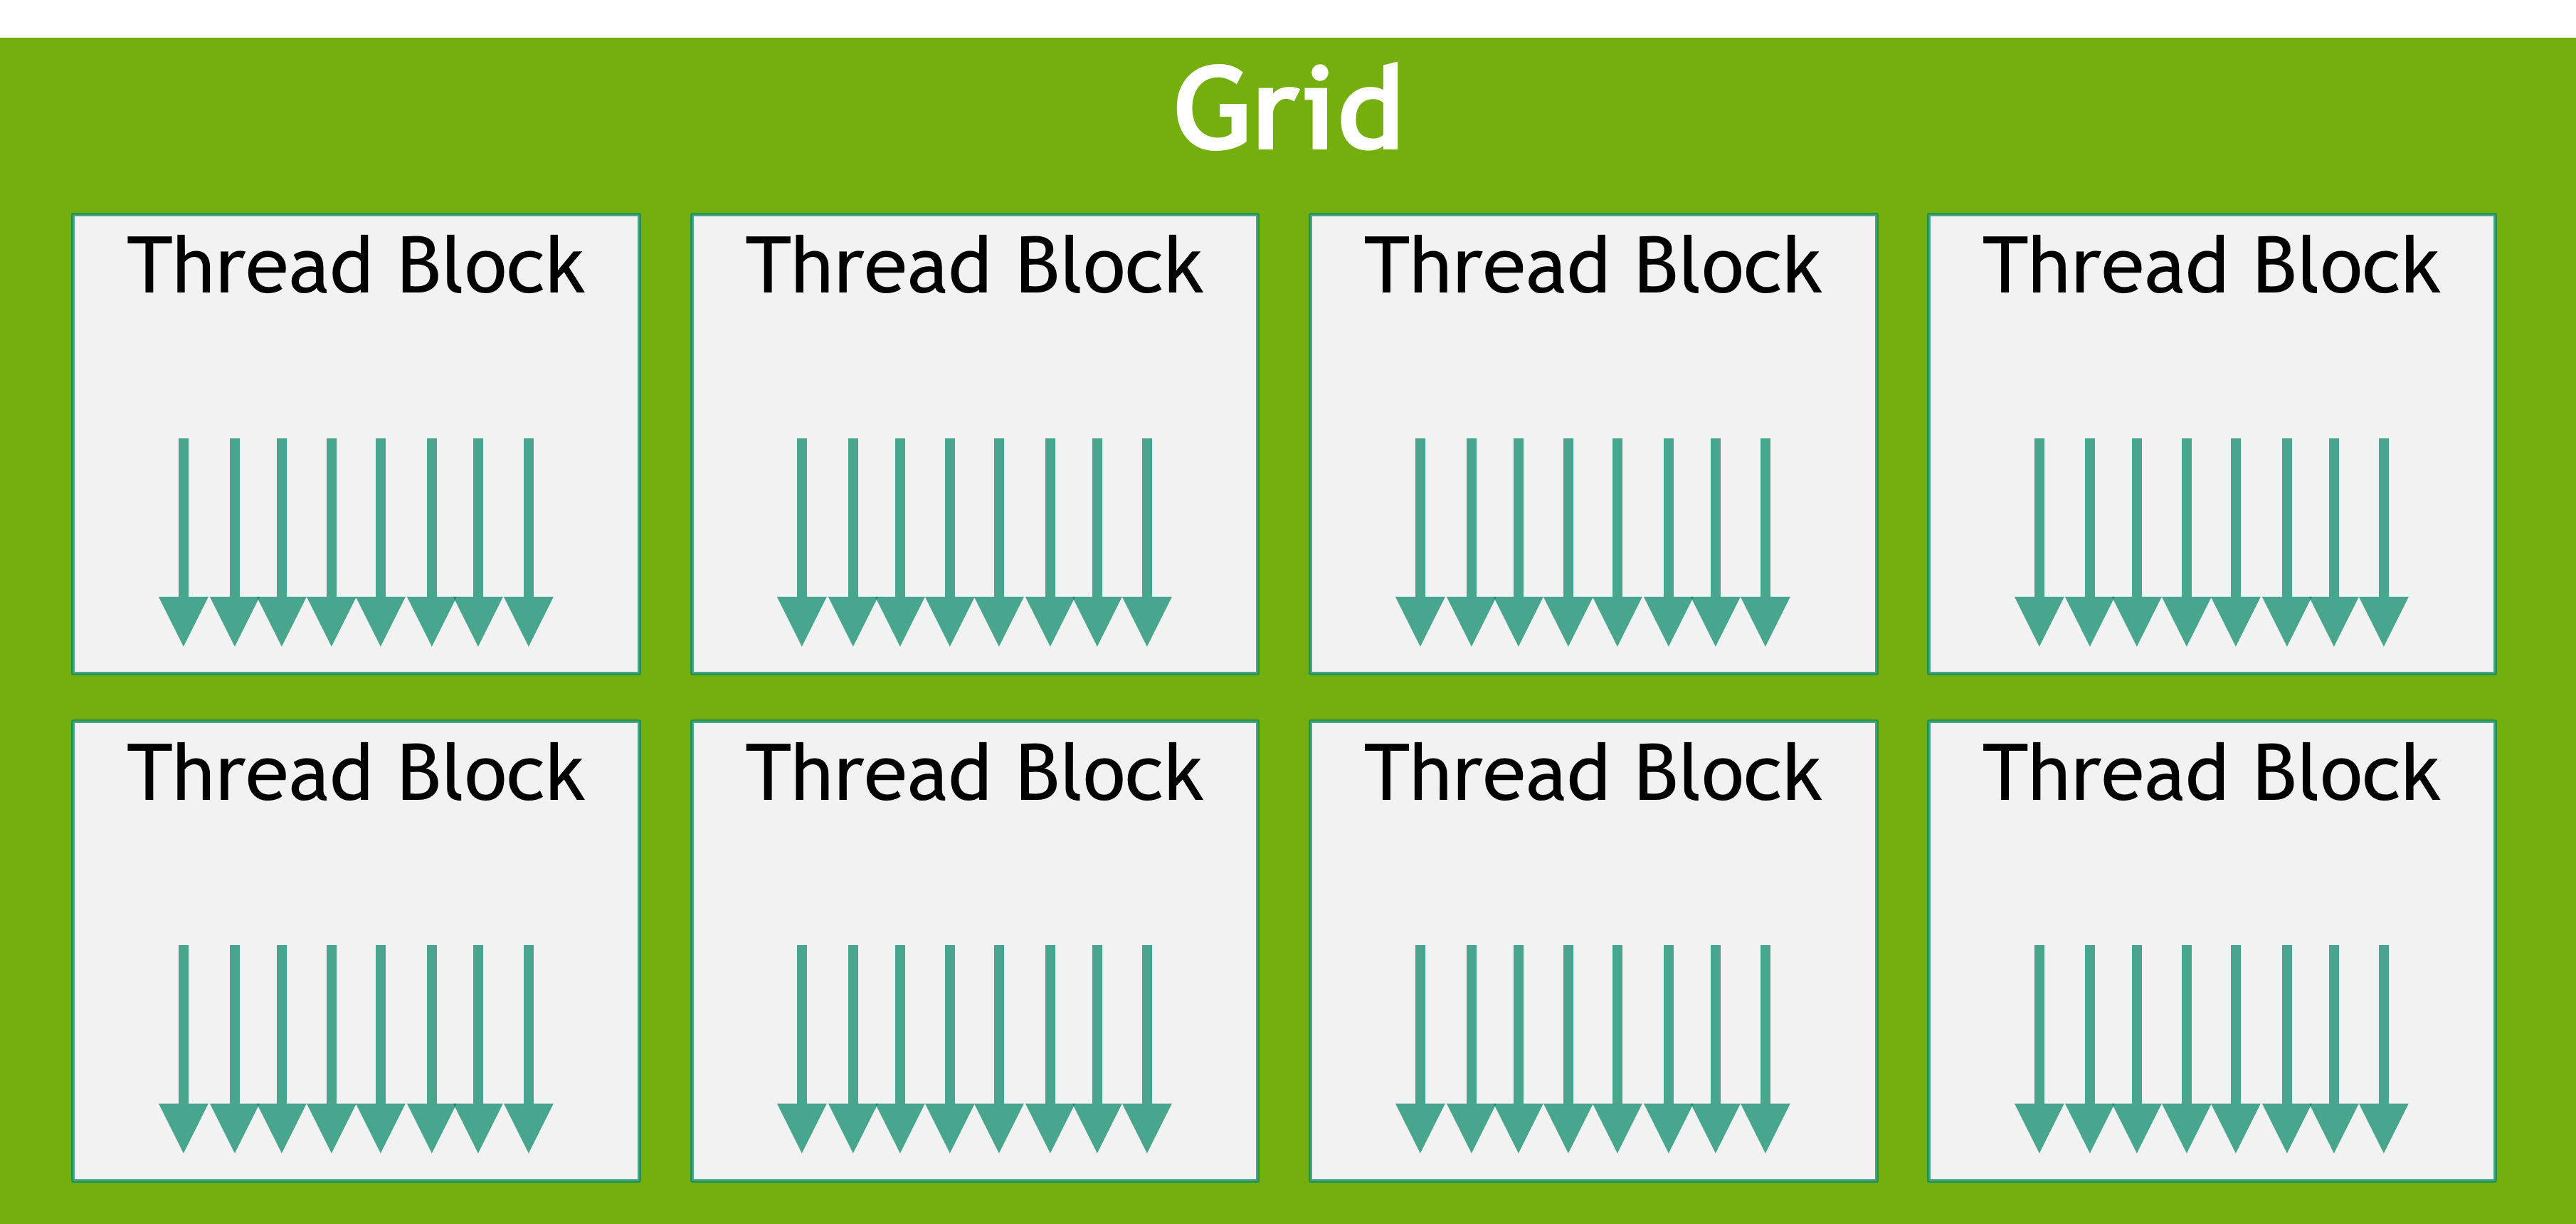
\includegraphics[width=0.7\textwidth]{src/images/grid-of-thread-blocks}
    \caption{Группа блоков формируют грид}\label{img:GridOfThreadBlocks}
\end{figure}


\subsubsection{Архитектура SIMT}

В CUDA аппаратной реализации видеокарт NVIDIA.

Микроархитектура графических процессоров общего назначения построена вокруг массива процессоров, называемых \textit{Streaming Multiprocessors (SMs)}. Когда происходит вызов CUDA кернела, блоки соответствующего грида нумеруются и распределяются между мультипроцессорами, учитывая доступные в данный момент времени вычислительные ресурсы. Количество одновременно исполняемых на мультипроцессоре блоков зависит от доступного объема регистрового файла и разделяемой памяти (англ. shared memory).

Мультипроцессор оперирует группой потоков фиксированного размера, называемой \textit{варп} (англ. \textit{warp}). Типичный размер варпа -- 32 потока. Перед попаданием в конвейер GPGPU вычислителя, CUDA блок разделяется на варпы. Количество варпов в блоке задается следующей тривиальной формулой:

\begin{equation}
    \text{Кол-во варпов в блоке} = \ceil[\bigg]{\frac{\text{Кол-во потоков в блоке}}{\text{Размер варпа}}}
\end{equation}

Все потоки в варпе одновременно исполняют одну и ту же инструкцию, поэтому максимальная утилизация вычислительных ресурсов происходит, когда все 32 потока согласованы на своем пути исполнения. Условный переход является одной их причин расхождения потоков в варпе (англ. intra-warp divergence). При расхождении, варп исполняет все ветви поочередно, деактивируя потоки, не принадлежащие данной ветви (см. рис. \ref{img:IntraWarpDivergence}).

\begin{figure}[!ht]
    \centering
    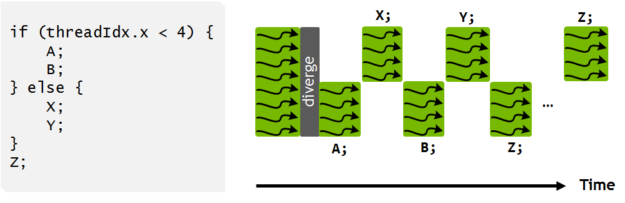
\includegraphics[width=0.7\textwidth]{src/images/intra-warp-divergence}
    \caption{Пример расхождения потоков в варпе}\label{img:IntraWarpDivergence}
\end{figure}